\normaltrue \difficilefalse \tdifficilefalse
\correctionfalse

%\UPSTIidClasse{11} % 11 sup, 12 spé
%\newcommand{\UPSTIidClasse}{12}
% ATS 2019
\exer{Suspension pneumatique de véhicule de transport routier $\star$ \label{A3:05:88}\label{SYS-01:A3:05:88}}
\setcounter{question}{0}
\marginnote{\xpComp{SYS}{01}}
\index{Compétence A3-05}
\index{Compétence SYS-01}
\index{Suspension pneumatique}
\index{Caractériser un constituant de la chaîne de puissance.}
\index{Distributeur}
\index{Vérin}
\ifcorrection
\else
\marginnote{\textbf{Pas de corrigé pour cet exercice.}}
\fi



\ifprof
\else
La suspension assure la liaison élastique entre le châssis et les essieux. Elle permet principalement d’atténuer les accélérations verticales dues aux variations de profil de la chaussée, contribuant ainsi à l’amélioration du confort et à une meilleure tenue de route.

\begin{marginfigure}
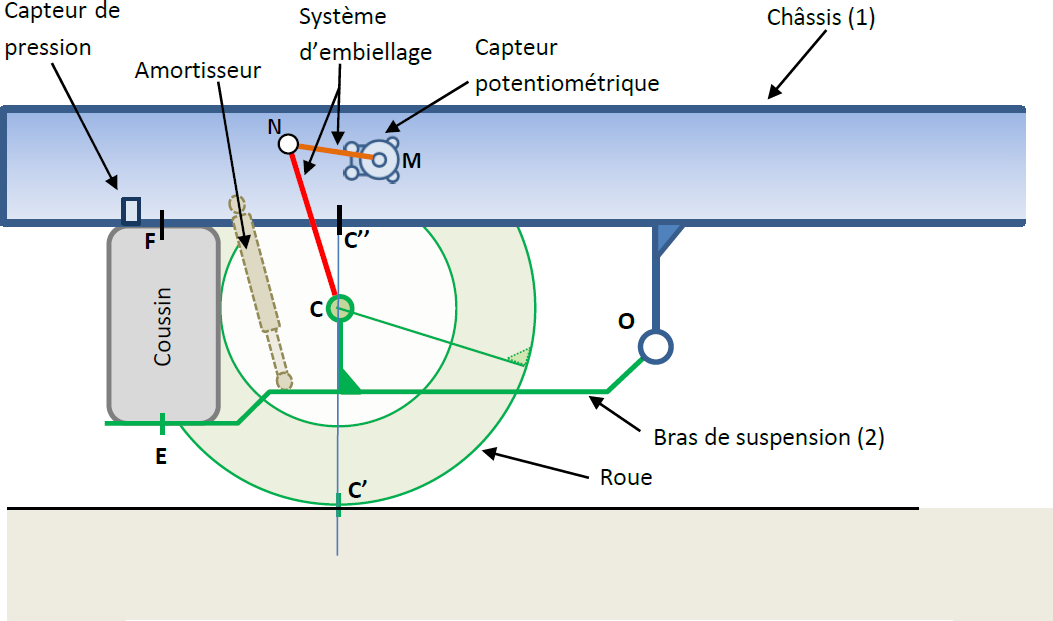
\includegraphics[width=\linewidth]{88_fig_01}
%\textit{}
\end{marginfigure}

Chaque roue possède une suspension pneumatique sur coussin pilotée par des électrovannes, en fonction de données mesurées par des capteurs de pression et des capteurs de position. Un calculateur envoie des commandes électriques aux électrovannes en fonction des besoins.

\begin{marginfigure}
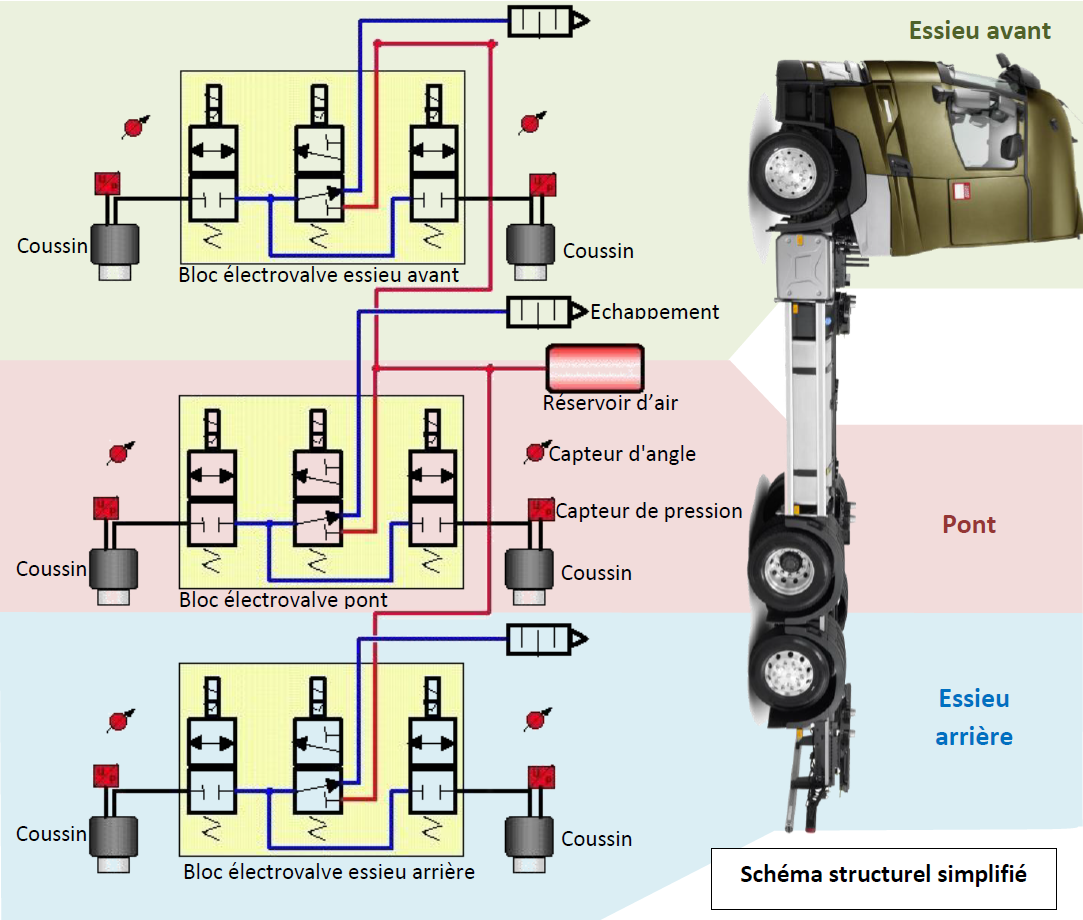
\includegraphics[width=\linewidth]{88_fig_02}
%\textit{}
\end{marginfigure}


\begin{center}
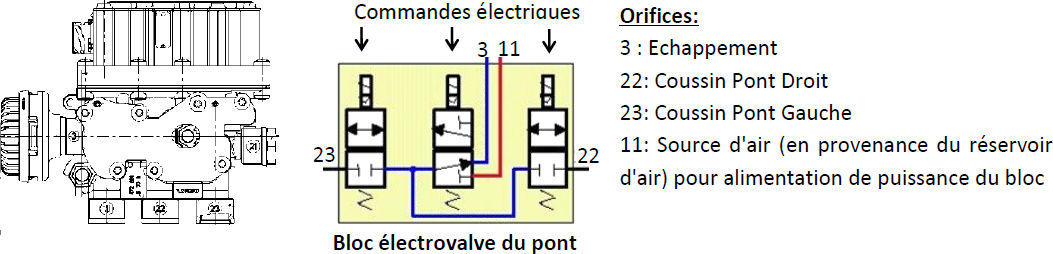
\includegraphics[width=\linewidth]{88_fig_03}
%\textit{}
\end{center}

Lorsque le niveau mesuré est inférieur à la valeur de consigne (niveau du châssis par rapport au sol), l’électrovalve est commandée de manière à provoquer le gonflage des coussins.
Lorsque le niveau a dépassé la consigne, on commande la vidange des coussins.

\fi
\question{Représenter les trois distributeurs dans la situation de gonflage, puis dans la situation de vidange des coussins.
}
\ifprof
\begin{marginfigure}
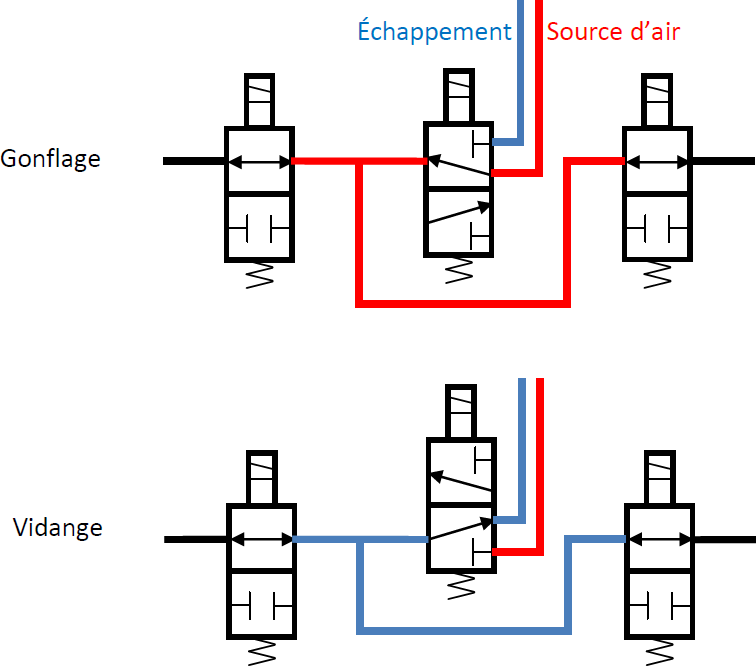
\includegraphics[width=\linewidth]{88_cor_01}
%\textit{}
\end{marginfigure}
\else
\fi

\ifprof
\else
\marginnote{Corrigé  voir \ref{A3:05:88}.}
\fi